\documentclass[11pt,a4paper]{amsart}
%\documentclass[paper=a4, fontsize=11pt]{scrartcl}
%\documentclass[12pt, final]{sreport}
\usepackage[utf8]{inputenc}
\usepackage[icelandic]{babel}
\usepackage[T1]{fontenc}
\usepackage{color}
\usepackage{amsmath, amsthm, amssymb, amsfonts}
\usepackage{enumerate}
\usepackage{url}
\usepackage{cite}
\usepackage{listings}
\usepackage{graphicx}
\usepackage{fancyhdr}
\usepackage{booktabs}
\usepackage{float}
\usepackage{hyperref}
\usepackage{caption}
\usepackage{subcaption}
\usepackage{setspace} 
\usepackage{lipsum}
\usepackage{ifthen}
\usepackage{geometry}

%\onehalfspacing
%\addtolength{\textheight}{2.4cm}
%\addtolength{\hoffset}{-1.2cm}
%\addtolength{\voffset}{-2cm}
%\addtolength{\textwidth}{2.3cm}

% Define new commands and operators
\newcommand{\N}{\mathbb{N}}
\newcommand{\No}{\N_0}
\newcommand{\Z}{\mathbb{Z}}
\newcommand{\perms}{\mathfrak{S}}

\DeclareMathOperator{\prst}{\mathcal{P}} 
\DeclareMathOperator{\rem}{rem}	
\DeclareMathOperator{\id}{id}
% End of new commands definitions

% Setup theorem styles
\theoremstyle{plain}
\newtheorem{theorem}{Theorem}[section]
\newtheorem{proposition}[theorem]{Proposition}
\newtheorem{lemma}[theorem]{Lemma}
\newtheorem{corollary}[theorem]{Corollary}
\newtheorem{conjecture}[theorem]{Conjecture}

\theoremstyle{definition}
\newtheorem{definition}[theorem]{Definition}
\newtheorem{example}[theorem]{Example}

\theoremstyle{remark}
\newtheorem*{remark}{Remark}
% End of theorem styles setup



\begin{document}

\newcommand{\HRule}{\rule{\linewidth}{0.5mm}}

\begin{titlepage}

\begin{center}
% Upper part of the page
%\includegraphics[width=0.55\textwidth]{rulogo.png}\\[4.0cm]    
%\includegraphics[width=4cm]{rulogo.png}

%\textsc{\LARGE Háskólinn í Reykjavík}\\[1.5cm]

\textsc{\LARGE Gagnavinnsla}\\[0.5cm]
\textsc{\Large Hópaverkefni 2}\\[0.6cm]

% Title
\HRule \\[0.4cm]
{ \Huge \bfseries MovieLens SQL database}\\[0.2cm]

\HRule \\[1.5cm]


% Author and supervisor
\begin{minipage}{0.49\textwidth}
\begin{flushleft} \large
\emph{Nemandi:}\\
Arnar Ingi Halldórsson\\
Halldór Stefánsson\\
Hjörleifur G. Bergsteinsson\\
Lárus Ívar Ívarsson\\
Þór Tómasarson
\end{flushleft}
\end{minipage}
\begin{minipage}{0.49\textwidth}
\begin{flushright} \large
\emph{Kennari:} \\
Eyjólfur Ingi Ásgeirsson
\end{flushright}
\end{minipage}

\vfill

% Bottom of the page
{\large \today}



\end{center}

\end{titlepage}

\section{Aðferð/Niðurstaða}
Í þessu verkefni fáum gögn með 10 milljón einkunnunum á 10,000 myndum frá 72,000 notendum.
Útfrá þessum gögnum eigum við annars vegar að finna topp 10 lista og hins vegar að setja fram spá sem segir til hvaða einkunn tilgreindur notandi myndi gefa tilgreindri kvikmynd og bera saman við einkunnina sem notandinn gaf myndinni ef einkunninn er til staðar.  
\\\par
Forritið byrjar á því að kanna hvort töflunar 'ratings', 'movies' og 'tags' séu í gagnagrunninum og býr þær til ef svo er ekki. Því næst býr forritið til töflu 'averageratings' í gagnagrunninum sem heldur utan um meðaltalseinkunn mynda, þar sem einkunnin er reiknuð út frá einkunnagjöf frá að lágmarki 100 notendum. Taflan 'averageratings' er gerð til að flýta fyrir framtíðar útreikningum. Þegar allar töflur eru komnar í gagnagrunninn kemur upp notendaviðmótið. Mynd~\ref{fig:schema} sýnir 'Database schema'.

\subsection{Topp 10}
Í notendaviðmótinu getur notandinn valið hvaða tegund(genre) af mynd og hversu stóran topplista notandinn vill og útfrá því fær notandinn topplista af þeirri tegund. Ef ekkert er valið, kemur topplisti yfir allar myndirnar.\par Þegar notandinn velur tegund leitum við í gagnagrunni 'movies.genre' með hjálp 'LIKE '\%genre\%'' skipunar í PostgreSQL. Forritið sækir upplýsingar um topplista í 'averageratings' töfluna. Sjá mynd~\ref{fig:top20}.

\subsection{Einkunnaspá}
Ef notandinn vill nýta sér einkunnaspánna getur hann annað hvort slegið inn sjálfur 'UserID' og 'MovieID' eða 'Movie Title' og þá fær hann spá frá tilgreindum einstaklingi fyrir valda bíómynd. Einnig getur hann valið 'UserID' og 'Movie Title' af handahófi. Einkunnarspá fyrir 'Much Ado About Nothing' má sjá á mynd~\ref{fig:predict}.\par
Til þess að setja fram spá finnum við út hvaða myndir valinn einstaklingur hefur gefið einkunn. Við finnum þá notendur sem hafa líka gefið þeim myndum einkunnir. Síðan nýtum við okkur einkunnagjöf þeirra notenda sem eiga flestar sameiginlega myndir með valda einstaklingnum. Lokaspáin er þá meðaltal þeirra einkunna sem þeir notendur hafa gefið valdri bíómynd. Gróf skýringarmynd um hvernig við hugsuðum spánna má sjá á mynd~\ref{fig:pdia}.


\subsection{BÓNUS - Mynd af handahófi}
Einnig erum við með smá auka valmöguleika, þar sem notandinn getur fengið upp mynd af handahófi eftir hvaða tegund og einkunnarskala hann vill.\par Þar notumst við eins og áður með hjálp 'LIKE '\%genre\%'' skipunar í PostgreSQL á 'movies.genre' gagnagrunninn og sækjum einkunnir í 'averageratings' töfluna.  Einnig er getur notandinn valið hvort hann vilji að IMDB slóð komi upp í vafranum. Mynd~\ref{fig:rad}.

\newpage

\section{Viðauki}
\vspace{2mm}
\begin{figure}[H]
	\centering
	\begin{subfigure}[H]{0.5\textwidth}
		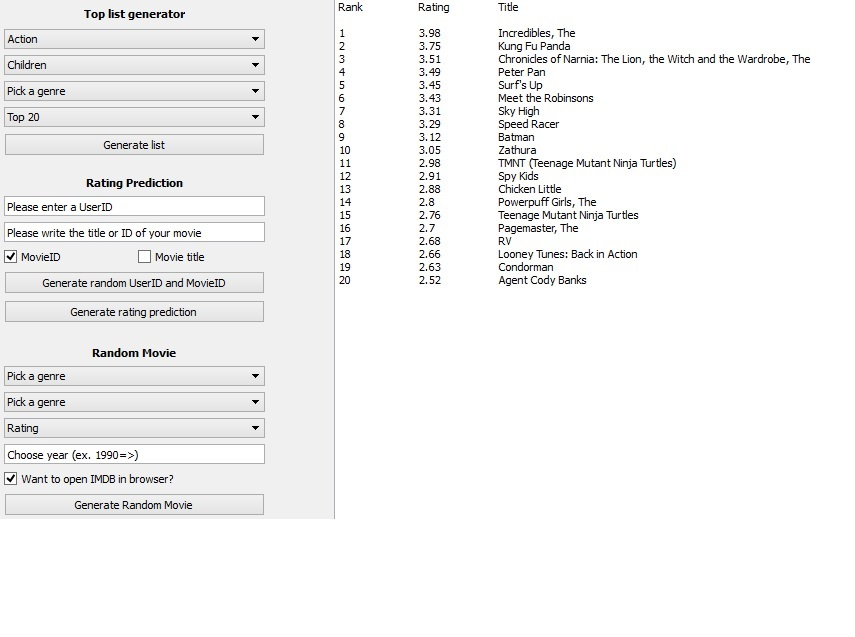
\includegraphics[height=50mm]{ui_top20.jpg}
		\caption{$ Topp\ 20\ listi $\label{fig:top20}}
	\end{subfigure}
	\begin{subfigure}[H]{0.4\textwidth}
		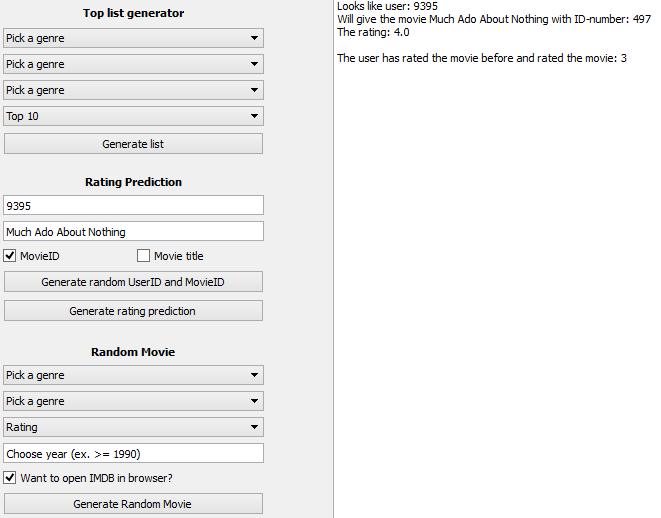
\includegraphics[height=50mm]{predict.png}
		\caption{$ Einkunnarspa\ fyrir\ Much\ Ado\ About\ Nothing$\label{fig:predict}}	
	\end{subfigure}
\end{figure}
\vspace{2mm}
\begin{figure}[H]
\centering
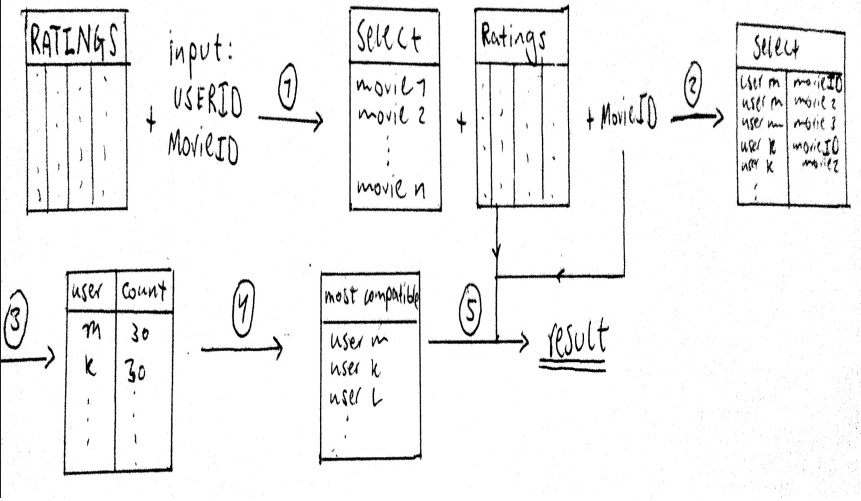
\includegraphics[height=50mm,width=16cm]{pre_dia.jpg}
\caption{$ Diagram\ fyrir\ einkunnarspa $\label{fig:pdia}}
\end{figure}
\vspace{2mm}

\begin{figure}[H]
	\centering
	\begin{subfigure}[b]{0.5\textwidth}
		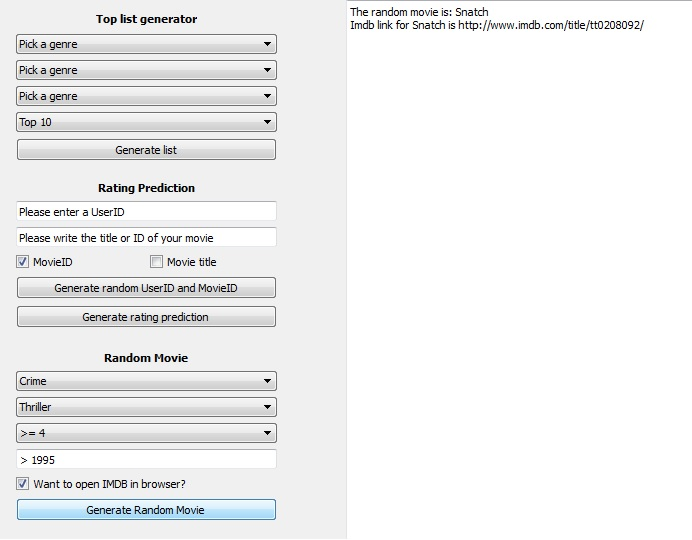
\includegraphics[height=50mm]{rand.jpg}
		\caption{$ Mynd\ af\ handahofi\ valin $\label{fig:rad}}
	\end{subfigure}
	\begin{subfigure}[b]{0.4\textwidth}
		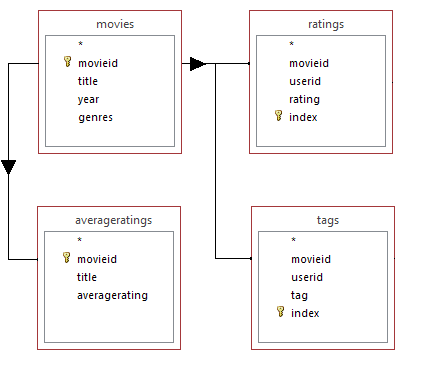
\includegraphics[height=50mm]{database_schema.png}
		\caption{$ Database\ schema $\label{fig:schema}}	
	\end{subfigure}
\end{figure}

\end{document}